\chapter{Музыка? Нет, не слышали\ldots}
\label{ch:music}

Сейчас мы зайдем на территорию искусства, вооружившись инструментами математики и физики. Читатель спросит: неужели мы сейчас начнем войну разума и чувств, науки и искусства? Нет и нет! Наоборот, мы будем наводить мосты дружбы между ними! 

Музыка отражает красоту математики, существующей \emph{внутри} нас, с помощью физики, существующей \emph{снаружи}. Музыка --- это один из способов передать математическую гармонию \emph{внутреннего} мира человека в несколько хаотичный \emph{окружающий} его мир.

А для тех, кто действительно не слышал музыку, дадим простое определение:

\begin{Definition}[Музыка]
    Музыка начинается тогда, когда звуки \emph{правильной} высоты с \emph{правильной} громкостью появляются в \emph{правильное} время
\end{Definition}

Давайте разбираться с музыкальными \emph{правилами}!


\section{Что да как? Немного физики}
\label{ch:music:physics}

Если задеть гитарную струну, вы услышите звук. Струна начнет колебаться и создавать вокруг себя периодические сжатия и разряжения воздуха, которые затем будут распространяться во все стороны от струны. Этот эффект называется звуковой \emph{волной}. По воздуху звуковая волна распространяется от источника со скоростью примерно\footnote{Скорость звука зависит от температуры, давления и влажности воздуха. В воде же звук распространяется гораздо быстрее} 340 метров в секунду.

Количество периодических сжатий (или разряжений) в секунду физики называют \emph{частотой}\footnote{Единица измерения частоты --- Герц. Сокращенно --- Гц. 1Гц --- одно колебание в секунду. 400Гц --- четыреста колебаний в секунду}, а лирики --- \emph{высотой} звука. Чем чаще колеблется струна, тем \emph{выше} звук, который она издаёт. Ну и наоборот: чем реже колеблется струна, тем \emph{ниже} звук. Верхние струны на гитаре (шестая, пятая и четвертая), издающие относительно низкие звуки, называются \emph{басовыми}.

Если вы дёрнете ту же струну сильнее, то она зазвучит \emph{громче}. При этом она издаст звук той же высоты, что и раньше. Но она будет совершать колебания с большим размахом --- физики скажут: <<с большей амплитудой>>. Сжатия и разряжения воздуха усилятся. И, когда звук дойдет до уха слушателя, эти сжатия и разряжения начнут сильнее шатать барабанную перепонку в его ухе и\ldots Тут физика кончится, и начнутся биология и биоинформатика.

Человеческое ухо может различать такие характеристики звуковой волны, как её частота и амплитуда. Незатухающие колебания одной неизменной частоты, человек услышит как тон\footnote{Например, заходящий на посадку на ваше ухо комар, машет крыльями примерно 659 раз в секунду и вы слышите незабываемое Ми второй октавы!}. А амплитуду волны (размах колебаний) --- как громкость. 

Человеческий слуховой аппарат воспринимает ограниченный диапазон частот --- примерно от 16 до 20000 Гц, а восприятие громкости звука, если честно, зависит не только от амплитуды звуковых колебаний, но и от частоты. 


\section{Как звучит струна? Правильная высота}
\label{ch:music:tone}

Если не менять натяжение и длину струны, то при игре она будет издавать звуки одной высоты (одного тона). Можно увеличить высту звука (увеличить частоту колебаний струны) двумя способами:
\begin{itemize}
    \item натянуть струну сильнее;
    \item укоротить струну, оставив натяжение прежним.
\end{itemize}

Перед игрой гитару настраивают, то есть регулируют определенным образом натяжение струн. В процессе игры натяжение отдельной струны не меняется. Гитарист извлекает звуки разной высоты, прижимая струну к разным металлическим порожкам лада, тем самым укорачивая её. Быстро и просто\footnote{Подробнее об устройстве гитары см. раздел \ref{ch:guitar}}.

На самом деле струна порождает не одну звуковую волну определенной частоты, а сразу бесконечное множество волн, потому что независимо друг от друга колеблются половинки струны, её трети, четверти и так далее!

\begin{figure}[!ht]
    \centering
    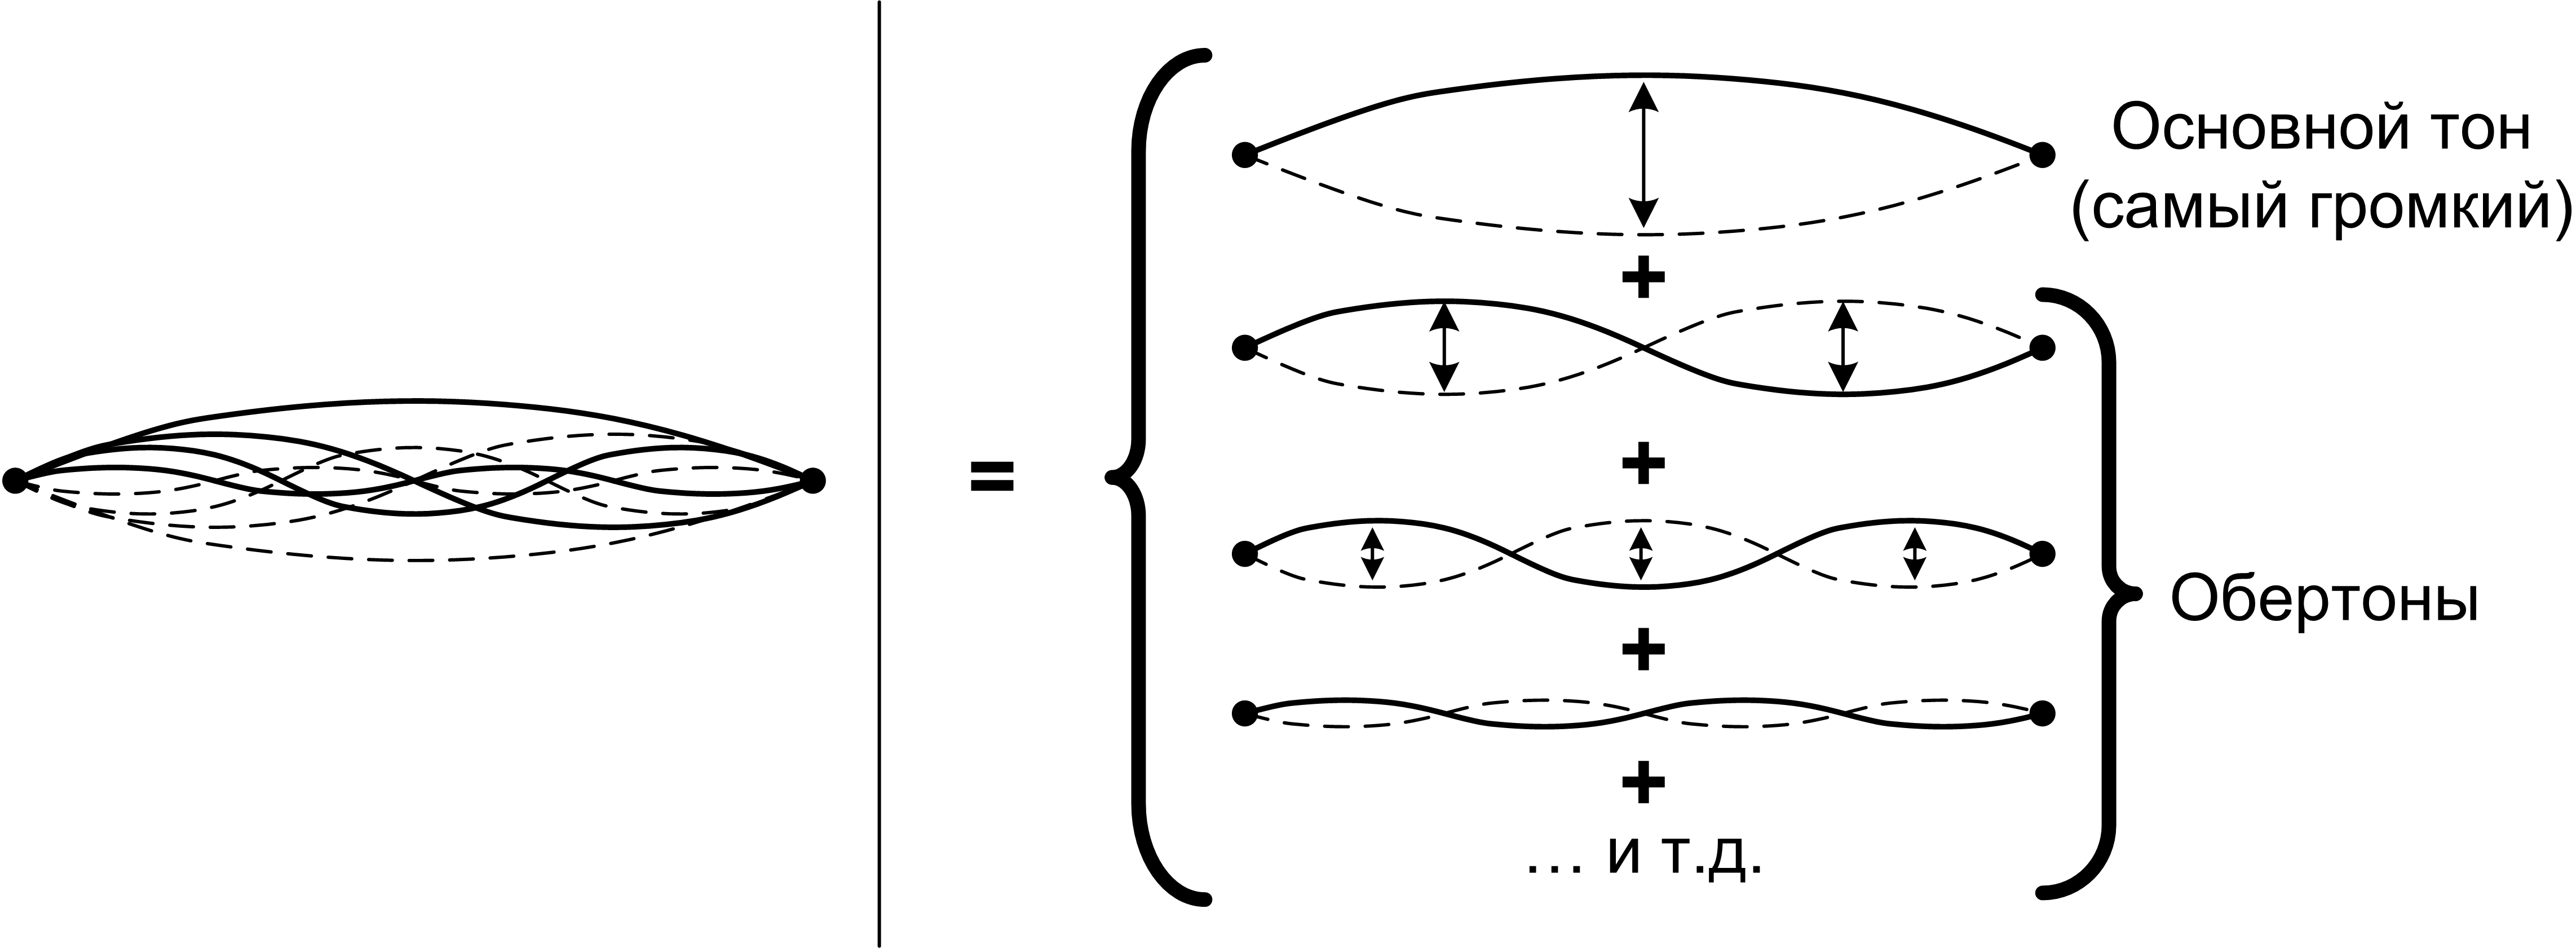
\includegraphics{fig/string-moving} 
    \caption{Колебания струны}\label{fig:music:tone:stringmoving}
\end{figure} 

На рисунке \ref{fig:music:tone:stringmoving} колебания струны разложены на составляющие (справа от знака равенства). Максимальную амплитуду колебаний имеет так называемый \emph{основной тон}, когда струна колеблется по всей длине. Основной тон слышен громче всех. Остальные составляющие принято называть \emph{обертонами}. Они звучат тише основного тона, но придают звуку особую окраску. Каждая гитара имеет свой особенный <<голос>> именно благодаря обертонам.

\begin{Definition}[Частота колебаний струны]
    Если при неизменном натяжении в $N$ раз \emph{укоротить} звучащую часть струны, то частота издаваемого основного тона \emph{увеличится} в $N$ раз.
\end{Definition}

Когда говорят о высоте звука струны, то по умолчанию имеют в виду именно частоту колебаний \emph{основного тона}.

Набор звуков различной высоты, которые можно извлечь из музыкального инструмента называется \emph{строем}. Чтобы создать гармонию, высота (частота) музыкальных звуков должна укладываться в строгую математическую систему. Таких систем (строев) сложилось несколько\footnote{Например, Чистый строй, Пифагоров строй}, но мы ограничимся только тем строем, который положен в основу конструкции гитары. Он называется <<равномерно-темперированным>>.

Прежде чем начать разбираться с равномерно-темперированным строем, нужно определить очень важное понятие: \emph{расстояние} между двумя звуками. То есть ввести меру отличия одного звука от другого по \emph{высоте}. 

Если укоротить струну вдвое, то частота её колебаний вдвое увеличится. Если взять такие звуки на открытой струне и на её половинке по отдельности, то вы легко уловите разницу между ними <<на слух>>. Если сыграть такие звуки одновременно, то они почти сольются: <<на слух>> один звук просто потеряется в другом. Это объяснимо: глядя на рисунок \ref{fig:music:tone:stringmoving} можно убедиться в том, что звук, издаваемый половинкой струны, полностью <<содержится>> в обертонах открытой струны. Самый громкий обертон имеет частоту вдвое меньшую, чем основной тон. 

\begin{Definition}[Октава]
    Два звука находятся друг от друга на расстоянии \emph{октавы}, если их частоты отличаются в два раза. Звук выше на октаву, если его частота в два раза больше частоты исходного звука. 
\end{Definition}

Ответ на вопрос: <<почему эта мера расстояния названа <<октавой>>?>> будет позже\footnote{Читайте раздел \ref{ch:harmony:interval}}. Октава --- это большое расстояние, а человеческое ухо воспринимает куда меньшие изменения частоты. Поэтому внимание: \emph{исторически} октаву делят на 12 кусочков. Такой кусочек называется <<полутоном>>.

\begin{Example}[Октава на грифе гитары]
    Давайте немного разбавим теорию практикой: возьмите гитару и линейку (можно даже просто суровую нитку). Измерьте длину любой струны (от верхнего порожка на грифе, до порожка на подставке, см. рисунок \ref{fig:guitar:construction}, если возникли трудности). Поделите длину струны на два (сложите нитку вдвое) и убедитесь, что середина струны находится над 12-м ладовым порожком. Звук, извлеченный на 12-м ладу, на \emph{октаву выше} звука открытой струны. Звук, извлеченный на 1-м ладу, \emph{выше} звука открытой струны на \emph{полутон}.
\end{Example}

В равномерно-темперированном строе частота от звука к звуку повышается в \emph{геометрической} прогрессии. То есть частота звука, который на полутон выше исходного, в \[\sqrt[12]{2}\approx 1,059463\] больше частоты исходного звука. В такой же пропорции находятся и расстояния между соседними ладовыми порожками гитары\footnote{Подробнее см устройство гитары в разделе \ref{ch:guitar}}.

Помимо способа задать расстояния между звуками, нужно также определиться с точкой отсчета. Международным стандартом зафиксировано, что эталонная частота, от которой ведется отсчет, составляет 440 Гц. Эта частота соотвествует ноте (подробно о нотах см. раздел \ref{ch:notes:names}) ЛЯ первой октавы. 

ЛЯ-диез первой октавы, который на полутон выше эталонного ЛЯ, имеет частоту $440\cdot\sqrt[12]{2}\approx 466,16$ герц. Эти различия ощущаются на слух. Звук СИ первой октавы (два полутона от эталонного ЛЯ) имеет частоту $440\cdot(\sqrt[12]{2})^2\approx 493,88$. И так далее, например, ЛЯ второй октавы (на 12 полутонов, то есть не октаву выше эталонного) имеет, как и положено, в два раза большую частоту: $440\cdot(\sqrt[12]{2})^{12}=440\cdot 2=880$ Гц.


\section{Маршируем или Вальсируем? Правильная громкость}
\label{ch:music:volume}

<<Аты-баты, шли солдаты, аты-баты на войну!>> Марш. Длительный пеший переход уныл без музыки. Ритм чеканим ногами: 
\begin{center}
    Левой--Левой--Раз-Два-Три-\ldots 
\end{center}
Знакомо? А что касается музыки, чтобы веселее шагалось, при наличии оркестра, лучше прям барабаном вжахнуть под левую ногу. Это называется \emph{акцентом}. 

<<Крутится, вертится шар голубой, Крутится, вертится над головой, Крутится, вертится, хочет упасть, Кавалер барышню хочет украсть>>. Вальс. 
\begin{center}
    Раз-два-три, Раз-два-три,\ldots 
\end{center}
В случае вальса какой-нибудь контрабас громко мурявкает на <<Раз>>.

Периодичность --- это часть нашей жизни. Пульсирует в жилах кровь, тикают секунды в часах, рассветы сменяются закатами, лето --- зимой. Вот и музыка пульсирует, живет акцентами. Живет по своему, где-то громче, где-то тише, и конечно живет не только вальсами и маршами.

Самый дешевый и сердитый способ сделать акцент на звуке --- выделить его громкостью. Обычный способ для гитары сделать акцент, не просто сильнее дернуть струну, а --- сыграть в унисон\footnote{В унисон - значит \emph{сливающимися} на слух звуками, читай раздел \ref{ch:music:tone}. То бишь отличающимися по частоте в два, четыре, восемь и т.д. раз} басом. Тяжелые басовые струны звучат громче.

Конечно, громкость --- не единственный способ сделать акцент. Звук может обратить на себя внимание, например, нестандартными обертонами (музыканты называют это \emph{тембровой} окраской звука). Сыграйте флажолет\footnote{О флажолете см. раздел \ref{ch:tricks:flageolet}} и оцените \emph{необычность} его звучания.


\section{Еще и глушить надо? Правильное время}
\label{ch:music:rythm}

Звуки сменяют друг друга и музыка течет во времени. 

Гитара позволяет извлекать несколько звуков сразу. Два звука, извлеченных одновременно\footnote{Ну, или очень быстро друг за другом. Например, при игре <<боем>> --- правая рука просто бъет вверх-вниз по всем струнам с определенным ритмом, а левая только успевает зажимать струны. При этом на каждый бой звучит аккорд, но струны, строго говоря, начинают звучать не одновременно}, называют \emph{интервалом}. Три и более --- \emph{аккордом}.

Интересно, что результат смешения звуков разной высоты, может быть как приянтым, так и неприятным на слух. Неприятное смешение звуков называется \emph{диссонансом}. Замечательно то, что заранее и абсолютно точно можно сказать как тот или иной интервал или аккорд повлияет на слушателя. Собственно музыка --- это искусство игры на нервах: создавая периоды приятных и неприятных звуковых ощущений, композитор добивается определенного настроения слушателя. Подробнее о теоретических основах гармонии мы поговорим позже, в главе \ref{ch:harmony}.

Колебания гитарной струны быстро затухают, то есть звук быстро теряет громкость. И чаще всего не нужно думать о том, чтобы заглушить струну: к тому моменту, когда вы извлечёте из гитары следующий звук, предыдущий потухнет сам. Но в музыкальном мире все относительно --- например, басовые струны звучат громче и дольше остальных, а стало быть их звук будет накладываться на на звуки, извлеченные позже. Если это будет приводить к диссонансам и это не предусмотрено композитором, то некоторые струны придется глушить, благо это несложно --- достаточно легко прикоснуться к струне пальцем.

Так как музыка пульсирует, укладывается в определенный ритм, создаваемый акцентами, то звуки действительно должны появиться в определенное время, чтобы поддержать эту пульсацию. В музыке введено понятие \emph{такта} --- фиксированного периода времени, через который обязательно появляются самые сильные акценты. И длительность отдельных звуков обычно измеряется долями такта, то есть звук может прозвучать: половину такта, четверть, восьмую долю, шестнадцатую и тд. Чаще всего такт делят степенями двойки, но нередко бывает, что звук длится треть такта, пятую или седьмую его часть.

Для буквоедов отметим, что звук, если его не заглушить специально, теоретически \emph{длится} (затухая) вечно. С практической же точки \emph{музыкальный} звук \emph{длится} до тех пор, пока не прозвучит куда более громкий следующий звук. 


\section{А радость где? Правильное отношение к правилам}
\label{ch:music:rules}

Правила существуют для того, чтобы их нарушать. Радость она ведь от озорства. Так что нарушать нужно искрометно и тонко, с хиртрецой. Так, чтобы вроде и нарушил, да ловко так, что и простить можно! Не закон Божий, в конце-то концов\ldots

Существует много озорных заигрыванй с правилами. Ну, например, приёмчик <<подтяжка>> струны: струна пальцем левой\footnote{Речь о правшах. Левши, вы знаете, что делать!} руки зажимается на ладу и играется как обычно, но, пока она звучит, палец, не ослабляя нажим, сдвигает (в пределах 1-2 см) струну вверх или вниз по порожку лада. Можно даже поелозить вверх-вниз. От таких действий натяжение струны меняется и звук плавно повышается, обычно в пределах долей полутона --- это уж как силушка богатырская позволяет. 

И таких хулиганств на гитаре придумано немало: всякие там вибратто, легато (hammer-on, pull-off), тэппинг и т.д. Забавно, что и вокруг хулиганств постепенно формируются свои правила: мол вот так <<подтяжку>> правильно играть, а так нет\ldots Ага, ага, не вопрос!

Заигрывают с ритмом, например, когда гитаристу вдруг захочется барабанов, он может побарабанить по гитаре --- фингерстайл\ldots Заигрывают и с длительностью звука, например, если электрогитару приблизить к усилителю звука, то усиленный звук струны, естественно звучаший в резонанс со струной, будет еще сильнее <<расшатывать>> струну, звук которой в свою очередь будет усилен. Обратная связь. Струна будет звучать (лучше сказать визжать) вечно, только ток на усилитель подавай!

Эх, прям на философию потянуло. Может потому-то и движется жизнь вперед? На месте хулиганств рождаются новые правила, порождающие очередные хулиганства. Обратная связь, ага. В общем без правил похулиганить не получится, а стало быть и радости никакой.

Напоследок: нарушать правила следует тогда, когда и знания, и мастерство позволяют это делать \emph{элегантно}.